\documentclass[a4paper,12pt]{article}
\usepackage[utf8x]{inputenc}
\usepackage[T1]{fontenc}
%\usepackage[T2A]{fontenc} % jei yra kirilica
\usepackage[hmargin={30mm,15mm},vmargin={20mm,20mm},bindingoffset=0mm]{geometry}
\usepackage[onehalfspacing]{setspace}
\usepackage[colorlinks=true, linkcolor=blue, citecolor=blue, urlcolor=blue, unicode]{hyperref}
%\parindent=7mm
\usepackage{graphicx}
\usepackage{caption}
\usepackage{float}
\usepackage{minipage-marginpar}
\usepackage{minted}
\usemintedstyle{default}
\newminted{python}{
	linenos=true,
	frame=none,
	bgcolor = bg,
	numbersep=5pt,
	fontsize=\footnotesize}
\renewcommand\listingscaption{Kodo fragmentas}
\renewcommand{\figurename}{Pav.}
%\renewcommand\listingscaption{pav.}

\renewcommand{\refname}{Literatūros sąrašas} % article
%\renewcommand{\bibname}{Literatūros sąrašas} % report
\renewcommand{\contentsname}{Turinys}
\begin{document}
\definecolor{bg}{rgb}{0.95,0.95,0.95}
\thispagestyle{empty} % nerasomas psl. nr

\begin{center}
 VILNIAUS UNIVERSITETAS 
 
MATEMATIKOS IR INFORMATIKOS FAKULTETAS

MATEMATINĖS INFORMATIKOS KATEDRA

\vspace{4cm}

\textbf{Vytautas Jankauskas} \ \ \textit{parašas}

Bioinformatikos studijų programa


\vspace{3cm}

\textbf{\Large Lietuviško rankraščio atpažinimas ir taikymas}

Bakalauro baigiamasis darbas 

\vspace{4cm}

Vadovas: lektorius \textbf{Irus Grinis} \ \   \textit{ parašas}

\vfill

Vilnius \ \  2017
\end{center}

\clearpage

\tableofcontents
\clearpage
%\maketitle 

\section*{Įvadas}
\addcontentsline{toc}{section}{Įvadas} % rasoma turinyje

\paragraph{}Kompiuteriu spausdinta ir ekrane matoma tekstinė medžiaga po truputį keičia žmonių rašymo ir skaitymo kultūrą bei yra naudojama vis plačiau. Tačiau ranka parašytas tekstas vis dar yra (ir tikriausiai visada bus) neatsiejama žmonių gyvenimo dalis. Tai ypač jaučiama švietimo įstaigose – mokyklose, kolegijose, universitetuose, kur svarbesnė informacija užrašoma ranka, kad būtų labiau išryškinta ir geriau įsiminta.

Žmonėms rega atrodo savaime suprantamas ir elementarus jutimo būdas. Jau ankstyvoje vaikystėje pradedama sąmoningai atpažinti įvairias spalvas, formas, objektus. Akimis matomas vaizdas smegenyse išskirstomas į įvairius signalus kuriais perduodama skirtingų tipų informacija. Pavyzdžiui, norint aptikti aplinkoje konkretų objektą, smegenys analizuoja tik svarbesnes, turinčias reikiamas savybes, matomo vaizdo dalis. Žmogus per savo gyvenimą apdoroja labai daug informacijos gaunamos visais jutimo organais. Ta informacija leidžia smegenims sukurti be galo daug įvairių sąryšių, padedančių atpažinti objektus.

Kompiuterinis vaizdinės medžiagos apdorojimas išsikelto tikslo įvykdymui yra vadinamas kompiuterine rega \cite{OPENCV}. Ji iš esmės turi tokią pat paskirtį kaip ir žmogaus rega. Tačiau kompiuteriai, skirtingai nei žmonės, vaizdinę medžiagą supranta tik kaip ilgą skaičių seką. Dirbtinės regos sistemos neturi jokio objektų atpažinimo modelio, nežino kurioje vietoje reikėtų fokusuoti vaizdą ar kurias jo dalis ignoruoti. Taip pat jos pačios neturi jokių sąryšių sistemų, kurios leistų palengvinti užduočių vykdymą. Taip pat bet kokiame vaizde egzistuoja įvairus triukšmas iš aplinkos, kurį sukuria kintantis apšvietimas, oro sąlygos.

Kompiuteriai visus su rega susijusius uždavinius gali išspręsti naudodami tik vaizdinę informaciją ir papildomą informaciją, kurią jiems suteikia žmonės tų užduočių įgyvendinimui. Kompiuterinė rega itin naudinga sprendžiant problemas, kurios iš žmonių reikalauja daug laiko, yra pasikartojančios. Todėl, nepaisant įvairių sunkumų, jos taikymų atsiranda vis daugiau:
\begin{itemize}
\item Pastaraisiais metais vis daugėja automatinio automobilių identifikacijos numerių atpažinimo sistemų. Kuriant tokias sistemas atsižvelgiama į įvairius veiksnius – numerių lokaciją, skaičių, kiekį, švarumą (lentelė su numeriais gali būti iš dalies padengta dulkėmis ar purvu), taip pat į apšvietimo sąlygas, vaizdo foną \cite{CARPLATE}.
\begin{figure}[H]
	\centering
	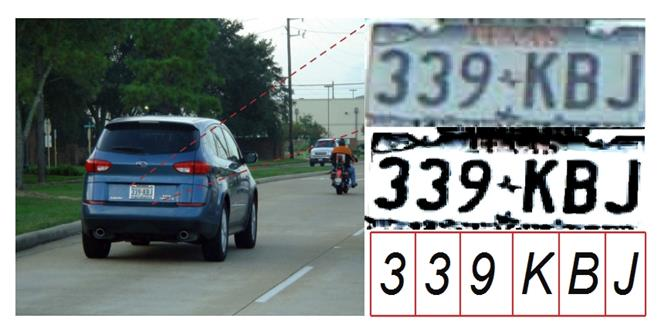
\includegraphics[scale=0.5]{images/carplate}
	\caption{Supaprastinta automobilių numerių atpažinimo schema \cite{PLATEIMG}.}   % Antraštė įterpiama po paveikslėlio
	\label{img:carplate}
\end{figure}
\item Vienas iš seniausių kompiuterinės regos taikymų yra pašto indeksų atpažinimas ant vokų ir siuntinių, leidžiantis sutaupyti daug laiko paštų darbuotojams \cite{POSTCODE}.
\begin{figure}[H]
	\centering
	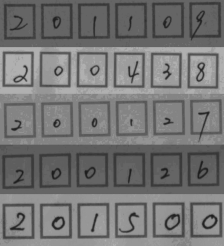
\includegraphics[scale=0.4]{images/postcode}
	\caption{Pašto indeksų pavyzdžiai iš Kinijos pašto.}   % Antraštė įterpiama po paveikslėlio
	\label{img:postcode}
\end{figure}
\item Beveik kiekvieno išmaniojo telefono kameroje yra galimybė naudoti veido aptikimo funkciją.
\item Vietose, kur renkasi dideli pėsčiųjų srautai, skaičiuojamas praeinančių žmonių kiekis. Tam naudojamos įprastos vaizdo kameros vaizdo srautą segmentuojant ir jame išskiriant kiekvieną žmogų atskirai \cite{PEOPLECOUNT}.
\item Sukurtas maliarijos diagnozavimo metodas, naudojant kompiuterinę regą \cite{MALARIA}. Gydytojui leidžia daug efektyviau dirbti, kadangi įrankis analizuoja kraujo mėginių atvaizdus ir atrenka tik tuos, kuriuose didžiausia maliarijos infekcijos tikimybė.
\end{itemize}

Šie pavyzdžiai rodo, kad kompiuterinės regos galimybės vis didėja, ją naudojančios sistemos tobulėja ir yra vis plačiau taikomos kasdieniame gyvenime. Ir vis dar egzistuoja daug problemų, prie kurių sprendimo galėtų prisidėti kompiuterinė rega. Įvairi programinė įranga gana lengvai atpažįsta spausdintas raides, skaičius ar kitus simbolius. Tą padaryti sąlyginai lengviau lyginant su ranka parašytais simboliais.

Lietuviškas rankraštis pasirinktas kaip bakalaurinio darbo temos objektas dėl to, jog jo atpažinimas ir taikymas gali būti panaudotas praktiškai Lietuvoje. Viena iš taikymo galimybių – palengvinti mokymosi procesą mokymo įstaigose sunkiau ar lėčiau besimokantiems mokiniams. Taip pat ir studentams, kuriems paskaitų metu kartais reikia spėti greitai užsirašyti didelius informacijos kiekius. Toks pritaikymo būdas leistų labiau susikoncentruoti į ugdytojo pateikiamą informaciją siekiant ją suprasti. Tuo pačiu metu būtų galima išsaugoti ranka užrašytą tekstą skaitmeniniu formatu ir jį vėliau panaudoti mokymosi tikslais.

Šio darbo tikslas:
\begin{itemize}
	\item Sukurti kompiuterinės programos, kuri atpažįsta lietuvišką rankraštį, prototipą. Programa turi gebėti iš nuotraukų su ant lentos užrašytu tekstu atpažinti ir vartotojui pateikti skaitmeninį teksto variantą.
\end{itemize}

Uždaviniai:
\begin{itemize}
	\item Susipažinti su kompiuterinės regos įrankiais naudojamais vaizdo normalizavimui, triukšmo pašalinimui.
	\item Susipažinti su elementariais mašininio mokymosi įrankiais ir algoritmais.
	\item Sukurti mokymosi duomenų aibę ir su ja apmokyti teksto atpažinimo algoritmą.
	\item Sukurti algoritmą, kuris nuskaito ir kuo tiksliau atpažįsta lietuvišką tekstą iš nuotraukos.
\end{itemize}

Teorinė šio darbo reikšmė yra sužinoti, kokios vaizdo apdorojimo procedūros ir įrankiai yra būtini norint normalizuoti atvaizdą, iš jo pašalinti aplinkos triukšmus. Įgyti bazines žinias apie duomenų rinkimą, paruošimą mašininio mokymosi algoritmams ir įgyti bazines žinias apie pačius algoritmus. Taip pat praplėsti supratimą apie panašių problemų sprendimus naudojantis kompiuterine rega.

Sukurti lietuvišką rankraštį atpažįstančios programos prototipą yra praktinė šio darbo reikšmė. Ši programa suteiktų galimybę greitai ir sklandžiai išsaugoti ranka parašytą tekstą skaitmeniniu formatu. Tai leistų ją panaudoti švietimo srityje moksleiviams, studentams. Taip pat darbas yra orientuotas į lietuvių kalbos rašmenis, todėl jis gali būti naudingas ir sprendžiant teksto vertimo į kitas kalbas problemas.

\clearpage

\section{Kompiuterinės regos biblioteka OpenCV}

Pagrindinis šio bakalauro darbo įrankis naudotas programos prototipo kūrimui yra OpenCV biblioteka \cite{CVWEB}. Ši biblioteka – vienas populiariausių įrankių kompiuterinės regos programoms kurti. Ji yra atvirojo kodo, turi aktyvią vartotojų bendruomenę. Biblioteką sudaro daugiau nei 2500 algoritmų, iš kurių daugiausia skirti vaizdų apdorojimui, taip pat mašininiam mokymui. Nors ir parašyta C++ programavimo kalba, OpenCV turi C, Python, Java ir MATLAB kalbų sąsajas taip dar palengvindama naudojimąsi. Taip pat palaikomos Windows, Linux, Mac OS ir Android operacinės sistemos. Daugiausiai naudojama kuriant realiu laiku veikiančias programas.

Buvo pasirinkta naudoti Python programavimo kalbos sąsają, kadangi ji yra paprasta naudoti ir darbo autorius jau turėjo patirties programuojant šia kalba. OpenCV biblioteka turi labai įvairių funkcijų ir pritaikymo būdų. Kadangi darbe buvo naudota tik nedidelė jų dalis, būtent jos yra apžvelgtos toliau.

\begin{itemize}
	\item Atvaizdo spalvų erdvės transformacijos. Spalvų erdvė yra metodas, kuriuo galima nustatyti, kurti ir atvaizduoti spalvas. Kiekvieną atvaizdą galima apibūdinti bet kurioje spalvų erdvėje \cite{COLORSPACE}. Priklausomai nuo išsikelto uždavinio, svarbu pasirinkti tinkamą spalvų formatą. Dažniausiai sutinkamas formatas, įprastas kompiuteriuose, televizoriuose, skaitmeninėse vaizdo kamerose yra RGB. Juo nurodoma, koks kiekis raudonos, žalios ir mėlynos spalvos reikalingas, norint atitikti konkrečią spalvą. Tuo tarpu HSV erdvė aprašomos spalvos pagal jose esantį pilkos spalvos kiekį ir pagal jų šviesumo stiprumą. Dar kompiuterinėje regoje dažnai naudojama ir pilkumo tonų (angl. grayscale) erdvė. Joje aprašoma tik juodos spalvos vertė. 
	\item  Kita svarbi dažnai naudojama vaizdo apdorojimo operacija yra atvaizdo slenksčio (angl. image threshold) nustatymas. Šio metodo metu kaip įvestis naudojamas paveikslėlis pilkumo tonų spalvų erdvėje. Jame, pagal pasirenkamą arba algoritmo nustatomą spalvos vertę kiekvienas taškas įgauna nulio arba vieneto vertę. Tai reiškia, kad už slenkstinę vertę didesnę vertę turintys taškai įgys juodos spalvos reikšmę, ir atvirkščiai.
	\begin{figure}[H]
			\centering
			
\includegraphics[scale=0.4]{images/threshold}
			\caption{Pilkumo tonų atvaizdas kairėje, slenkstinis – viduryje. Invertuotas slenkstinis – dešinėje \cite{THRESHOLD}.}   % Antraštė įterpiama po paveikslėlio
			\label{img:threshold}
	\end{figure}
	
	\item Vartotojo veiksmų fiksavimas, konkrečiau – paspaustų mygtukų fiksavimas yra dar viena OpenCV bibliotekos funkcija, kuria naudotis labai paprasta.
	\begin{listing}[H]
		\begin{pythoncode}
			# Importuoti OpenCV biblioteką:
			import cv2

			# Kintamajam key priskiriame pirmo paspausto mygtuko reikšmę
			key = cv2.waitKey(0)
			# Jei vartotojas paspaudžia "Enter", išspausdinti:
			if key == 13:
				print("Paspaudėte Enter.")
		\end{pythoncode}
	\begin{center}
		1 kodo fragmentas. Mygtukų paspaudimo naudojimo pavyzdys.
	\end{center}		
	\end{listing}
	
	\item Morfologinės transformacijos yra paprastos operacijos, atliekamos remiantis atvaizdo forma. Dažniausiai šioms operacijoms atlikti naudojami binariniai atvaizdai. Kaip įvesties elementai morfologinėms transformacijoms naudojamas norimas atvaizdas ir papildomas struktūrinis elementas, kuris ir nusprendžia, kaip bus vykdoma operacija. Struktūrinis elementas išties yra kvadratinė matrica, dažniausiai užpildyta vienetais. Pagrindinės operacijos yra ardymas (angl. erosion) ir išplėtimas (angl. dilation).
	
	Ardymo operacija veikia panašiai kaip ir dirvožemio ardymas, tik ji ardo atvaizdo priekinio plano objekto kraštus. Struktūrinis elementas slenkamas per paveikslėlio taškus. Originaliam paveikslėlio taškui (turinčiam vertę 0 arba 1) bus priskiriama vertė 1 tik tuo atveju, jei visi taškai po struktūriniu elementu bus lygūs 1. Kitu atveju paveikslėlio taškui priskiriama 0 vertė (jis suardomas). Taip sumažinamas priekinio vaizdo objekto plotas.
			\begin{figure}[H]
				\centering
				
\includegraphics[scale=0.5]{images/erosion1}
				\caption{Kairėje – originalus atvaizdas. Dešinėje – po ardymo operacijos.}   % Antraštė įterpiama po paveikslėlio
				\label{img:erosion1}
			\end{figure} 
	
	Išplėtimo operacija yra atvirkščia ardymui. Šiuo atveju, jei bent viena taško vertė struktūriniame elemente yra lygi vienam, tuomet ir originalus taškas atvaizde bus lygus vienam. Taigi, šiuo metodu išplečiame priekinio vaizdo objekto plotą. Dažniausiai, kai norima sumažinti triukšmą paveikslėlyje, po ardymo vykdomas išplėtimas. Taip ardymas pašalina baltus triukšmo taškus atvaizde, bet ir sumažina priekinio objekto plotą. Tam, kad objekto plotas vėl padidėtų, atliekamas išplėtimas, bet bet triukšmas nebeatsiranda iš naujo.
				\begin{figure}[H]
					\centering
					
\includegraphics[scale=0.5]{images/dilation}
					\caption{Kairėje – originalus atvaizdas. Dešinėje – po išplėtimo operacijos.}   % Antraštė įterpiama po paveikslėlio
					\label{img:dilation}
				\end{figure} 
	
	\item Mašininio mokymo algoritmai. OpenCV biblioteka turi funkcijų įvairioms mašininio mokymo operacijoms atlikti – statistinius modelius, kNN (angl. K–Nearest Neighbors) algoritmą, SVM (angl. Support Vector Machine) algoritmą, sprendimų medžių, atsitiktinių medžių algoritmus, neuroninius tinklus ir kitus.
	
	Plačiau apžvelgiamas kNN algoritmas. Jis yra vienas paprasčiausių klasifikacijos algoritmų naudojamų prižiūrimam mokymui (angl. supervised learning). Pagrindinė algoritmo idėja yra ypatybių erdvėje surasti artimiausią atitikmenį testiniams duomenims \cite{KNN}. Pav. 4 dvi skirtingas duomenų klases vaizduoja mėlyni kvadratai ir raudoni trikampiai. Kiekvienas duomuo turi po 2 ypatybes (grafike tai parodo x ir y koordinatės ir taško pozicija). Naujas testinis duomuo yra žalias apskritimas. Tad proceso, vadinamo klasifikacija metu algoritmas turi nuspręsti, kuriai duomenų klasei jį priskirti. Jei žiūrima tik į vieną artimiausiai esantį kaimyną, tai testinis duomuo būtų priskirtas raudonų trikampių klasei (kaip ir jei ieškoma 2 artimiausių kaimynų). Klasifikuojant pagal 3 kaimynus, duomuo vis tiek būtų priskirtas raudonųjų klasei. Naudojant šį algoritmą nereikėtų rinktis lyginio kaimynų skaičiaus, nes tuomet rezultatas gali būti lygus ir reikėtų ieškoti kitų savybių norint teisingai klasifikuoti. Pasirinkus 5 ar daugiau kaimynų, matoma, kad tokiu atveju žaliasis apskritimas būtų priskirtas mėlynųjų klasei. Toks klasifikavimas žiūrint į duomenų išsidėstymą atrodo teisingas.
		\begin{figure}[H]
			\centering
			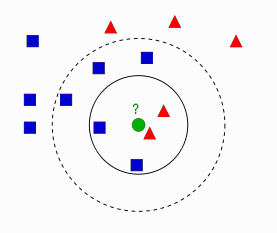
\includegraphics[scale=0.6]{images/knn}
			\caption{kNN algoritmo vizualizacija 2 duomenų klasėse.}   % Antraštė įterpiama po paveikslėlio
			\label{img:knn}
		\end{figure}
	Galima tarti, kad kNN algoritmui įtaką daro tik artimiausių kaimynų skaičius. Tačiau, būtina paminėti, kad klasifikuojant kiekvieną naują duomenų aibės narį, esamiems duomenims priskiriami skirtingi svoriai. Jie nustatomi pagal atstumą iki naujojo nario. Remiantis šia savybe, galima tarti, kad klasifikuojant pav. 4 grafike esantį žalią apskritimą pagal 4 artimiausius kaimynus, jis būtų priskirtas raudonųjų trikampių klasei, kadangi šie yra arčiau nei mėlynieji kvadratai.
\end{itemize} 

\subsection{A1 pavadinimas}
 Tekstas ...
 \subsection{A2 pavadinimas}
 Tekstas su formule $y=x^2$...
 
 %Paveikslas (jpg, png, pdf ir kiti formatai, jei kompiliuojate
 %su pdflatex):
%\[
%\includegraphics[scale=0.8]{mif-logo.png}
%\] 
 
 \section{Problemos sprendimas}

\paragraph{} Norint sukurti programos, gebančios atpažinti lietuvišką rankraštį, prototipą ir jį pritaikyti, buvo pasirinkta Python programavimo kalba. Naudojantis įvariais kalbos moduliais bei OpenCV kompiuterinės regos biblioteka atlikti išsikelti uždaviniai ir įgyvendintas pagrindinis darbo tikslas – sukurtas ir praktiškai išbandytas prototipas. Šiame skyriuje aprašomas uždavinių sprendimas, jų rezultatai, kilusios problemos, pastabos ir pasiūlymai. 

\subsection{Pradinis vaizdo apdorojimas}
 \paragraph{} Norint išbandyti tinkamą programos prototipo veikimą, iš pradžių būtina turėti kokybiškos vaizdinės medžiagos. Todėl šiame darbe naudota vaizdinė medžiaga buvo fiksuojama esant geroms, pastovioms apšvietimo sąlygoms. Tokiu būdu norėta išvengti papildomo triukšmo paveikslėliuose. Taip pat buvo stengiamasi išrinkti pakankamai kontrastingus priekinio plano objektus ir foną atvaizduose.
 
 Darbe naudojami atvaizdai pirmiausiai įkeliami į programą naudojant OpenCV bibliotekos funkcijas. Taip pat sumažinama jų skiriamoji geba.
\begin{listing}[H]
	\begin{pythoncode}
		# Importuoti OpenCV biblioteką:
		import cv2
		# Įkelti atvaizdą į programą:
		img = cv2.imread('gb3.png')
		# Sumažinti skiriamąją gebą:
		newx,newy = img.shape[1]/3.5,img.shape[0]/3.5
		newimage = cv2.resize(img,(int(newx), int(newy)))
	\end{pythoncode}
	\begin{center}
		2 kodo fragmentas. Atvaizdo įkėlimas į programą.
	\end{center}		
\end{listing}



   
 \subsection{B2 pavadinimas}
 Poskyris B2 turi du skirsnius
 \subsubsection{B21 pavadinimas}
  Tekstas....
  \subsubsection{B22 pavadinimas}
  Tekstas....
 \subsection{B3 pavadinimas}
 Tekstas su nauja formule $y=x^3$...
 
 
\begin{thebibliography}{99}
\addcontentsline{toc}{section}{Literatūra} %% Literatura bus itraukta i turini
\bibitem {OPENCV}
G. Bradski ir A. Kaehler, \textit{Learning OpenCV: Computer vision with the OpenCV library}, O'Reilly Media, Inc., 2008, p. 1–8.

\bibitem {MALARIA}
N. Linder, ir kt., \textit{A malaria diagnostic tool based on computer vision screening and visualization of Plasmodium falciparum candidate areas in digitized blood smears}, PLoS One 9.8 (2014): e104855.

\bibitem {CARPLATE}
E. Christos-Nikolaos Anagnostopoulos ir kt., \textit{License plate recognition from still images and video sequences: A survey} IEEE Transactions on intelligent transportation systems 9.3 (2008), p. 377-391.

\bibitem {PRADEEP}
J. Pradeep, E. Srinivasan ir S. Himavathi, \textit{Diagonal based feature extraction for handwritten character recognition system using neural network}, Electronics Computer Technology (ICECT), 2011 3rd International Conference IEEE, 2011.

\bibitem{PEOPLECOUNT}
C. Chen ir kt., \textit{A cost-effective people-counter for a crowd of moving people based on two-stage segmentation}, Journal of Information Hiding and Multimedia Signal Processing 3.1 (2012): 12-25.
 
\bibitem {LeCun}
Y. LeCun ir kt., \textit{Comparison of learning algorithms for handwritten digit recognition}, Tarptautinė neuroninių tinklų konferencija, 1995.
\url{http://yann.lecun.com/exdb/publis/pdf/lecun-95b.pdf}

\bibitem{PLATEIMG}
D. Kostadinov, \textit{Privacy Implications of Automatic License Plate Recognition Technology}, \url{http://resources.infosecinstitute.com/privacy-implications-automatic-license-plate-recognition-technology/}.

\bibitem{POSTCODE}
 Shujing Lu ir kt., \textit{Cost-sensitive neural network classifiers for postcode recognition}, International Journal of Pattern Recognition and Artificial Intelligence, 2012.
 
\bibitem{CVWEB}
OpenCV kompiuterinės regos bibliotekos žiniatinklio puslapis, \url{http://opencv.org/about.html}

\bibitem{CVCOLORS}
OpenCV spalvų erdvės transformacijos, \url{http://docs.opencv.org/3.2.0/df/d9d/tutorial_py_colorspaces.html}

\bibitem{COLORSPACE}
A. Ford, Alan Roberts, \textit{Colour Space Conversions}, 1998
\url{http://sites.biology.duke.edu/johnsenlab/pdfs/tech/colorconversion.pdf}

\bibitem{THRESHOLD}
Atvaizdo slenkstinės vertės nustatymas, \url{http://docs.opencv.org/trunk/d7/d4d/tutorial_py_thresholding.html}

\bibitem{KNN}
kNN algoritmo paaiškinimas, \url{http://opencv-python-tutroals.readthedocs.io/en/latest/py_tutorials/py_ml/py_knn/py_knn_understanding/py_knn_understanding.html#knn-understanding}


\end{thebibliography} 
 
 
\section*{Santrauka}
\addcontentsline{toc}{section}{Santrauka}
Trumpa darbo santrauka...
\section*{Summary}
\addcontentsline{toc}{section}{Summary}
Short english summary... 



\end{document}
